\documentclass[11pt,a4paper]{article}
\usepackage[utf8]{inputenc}
\usepackage[german]{babel}
\usepackage{amsmath}
\usepackage{amsfonts}
\usepackage{subfig}
\usepackage{amssymb}
\usepackage{siunitx,physics}
\usepackage{mathtools}
\usepackage{graphicx}
%\usepackage{Here}
\usepackage[version=4]{mhchem}
\usepackage{url}
\usepackage{setspace}
\usepackage[left=2.5cm,right=2.5cm,top=2.5cm,bottom=2cm]{geometry}
[biblography=totocnumbered]
\usepackage{fancyhdr}
\usepackage{scrextend}
\usepackage{hyperref}
\pagenumbering{gobble}

\makeatletter
\newcommand\bigcdot{\mathpalette\bigcdot@{.5}}
\newcommand\bigcdot@[2]{\mathbin{\vcenter{\hbox{\scalebox{#2}{$\m@th#1\bullet$}}}}}
\makeatother

\makeatletter
%\renewcommand*\bib@heading{%
%  \subsection*{}%
%  \@mkboth{\refname}{\refname}}
%\makeatother
\numberwithin{equation}{section}
\numberwithin{figure}{section}

\renewcommand{\labelitemii}{\labelitemfont$\vartriangleright$}
\begin{document}\\
\begin{addmargin}[25pt]{0pt}    
Man unterscheidet bei den Liniendefekten zwischen der Stufenversetzung und der Schraubenversetzung. Die Stufenversetzung ist in Abbildung \ref{fig:Stufenversetzung} dargestellt. Bei ihr wird eine zusätzliche Halbebene in den Kristall eingefügt welche mit einer Stufe abrupt endet. Das Gitter wird aufgrund dieser zusätzlichen Ebene verzerrt. Die Schraubenversetzung, siehe Abbildung \ref{fig:Schraubenversetzung} beschreibt den Fehler, dass der obere Teil des Kristalls um einen Atomabstand verschoben ist. 

\begin{figure}[h]
  \centering
  \subfloat[Visualisierung einer Stufenversetzung\label{fig:Stufenversetzung}]{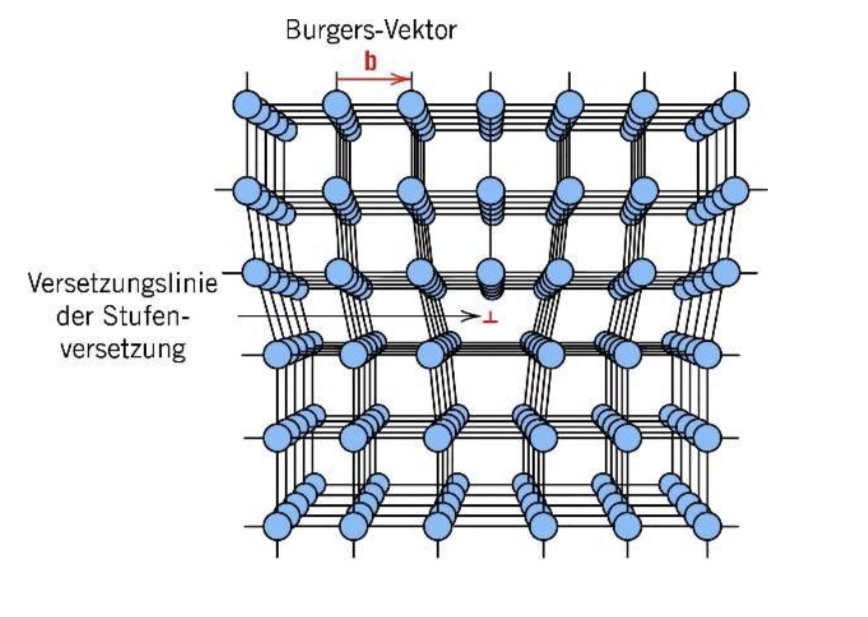
\includegraphics[height = 5cm,width=5cm]{images/Materialwissenschaften/Stufenversetzung.jpeg}}\qquad
  \subfloat[Visualisierung einer Schraubenversetzung\label{fig:Schraubenversetzung}]{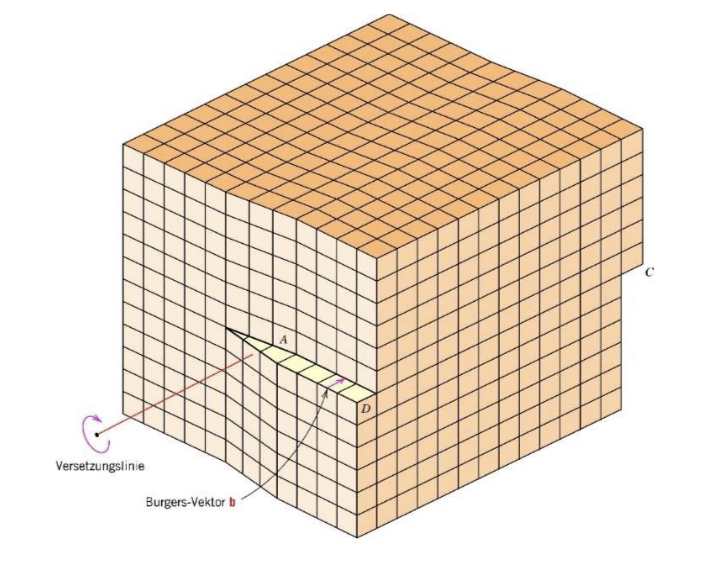
\includegraphics[height =5cm, width=5cm]{images/Materialwissenschaften/Schraubenversetzung.jpeg}}
\caption{Stufenversetzung und Schraubenversetzung}
\label{fig:Liniendefekte}
\end{figure}

\end{addmargin}

\end{document}